


%--------------------------------------------------------------------------------------------------------------------

\section {Sensitivity study for larger number of POT}
\label{subsec:future_sensi}

A sensitivity study for future number of POT is performed.
In 1 year we expect to collect data statistic for about \FuturePot POT.
The expected number of events as well as the rate-only and rate+shape
p-values are shown respectively for \FakePotLow POT, \FakePotHigh POT,
$6.5 \times 10^{20}$ POT, $8.0 \times 10^{20}$ POT and $9.0 \times 10^{20}$ POT
in figure~\ref{fig:sensi_future_nobs} and figure~\ref{fig:sensi_future_pvalue}.
In order to reach a significance corresponding to a p-value of 0.02-0.01 
we need to collect about $9.0 \times 10^{20}$ POT.

\begin{figure}
\center
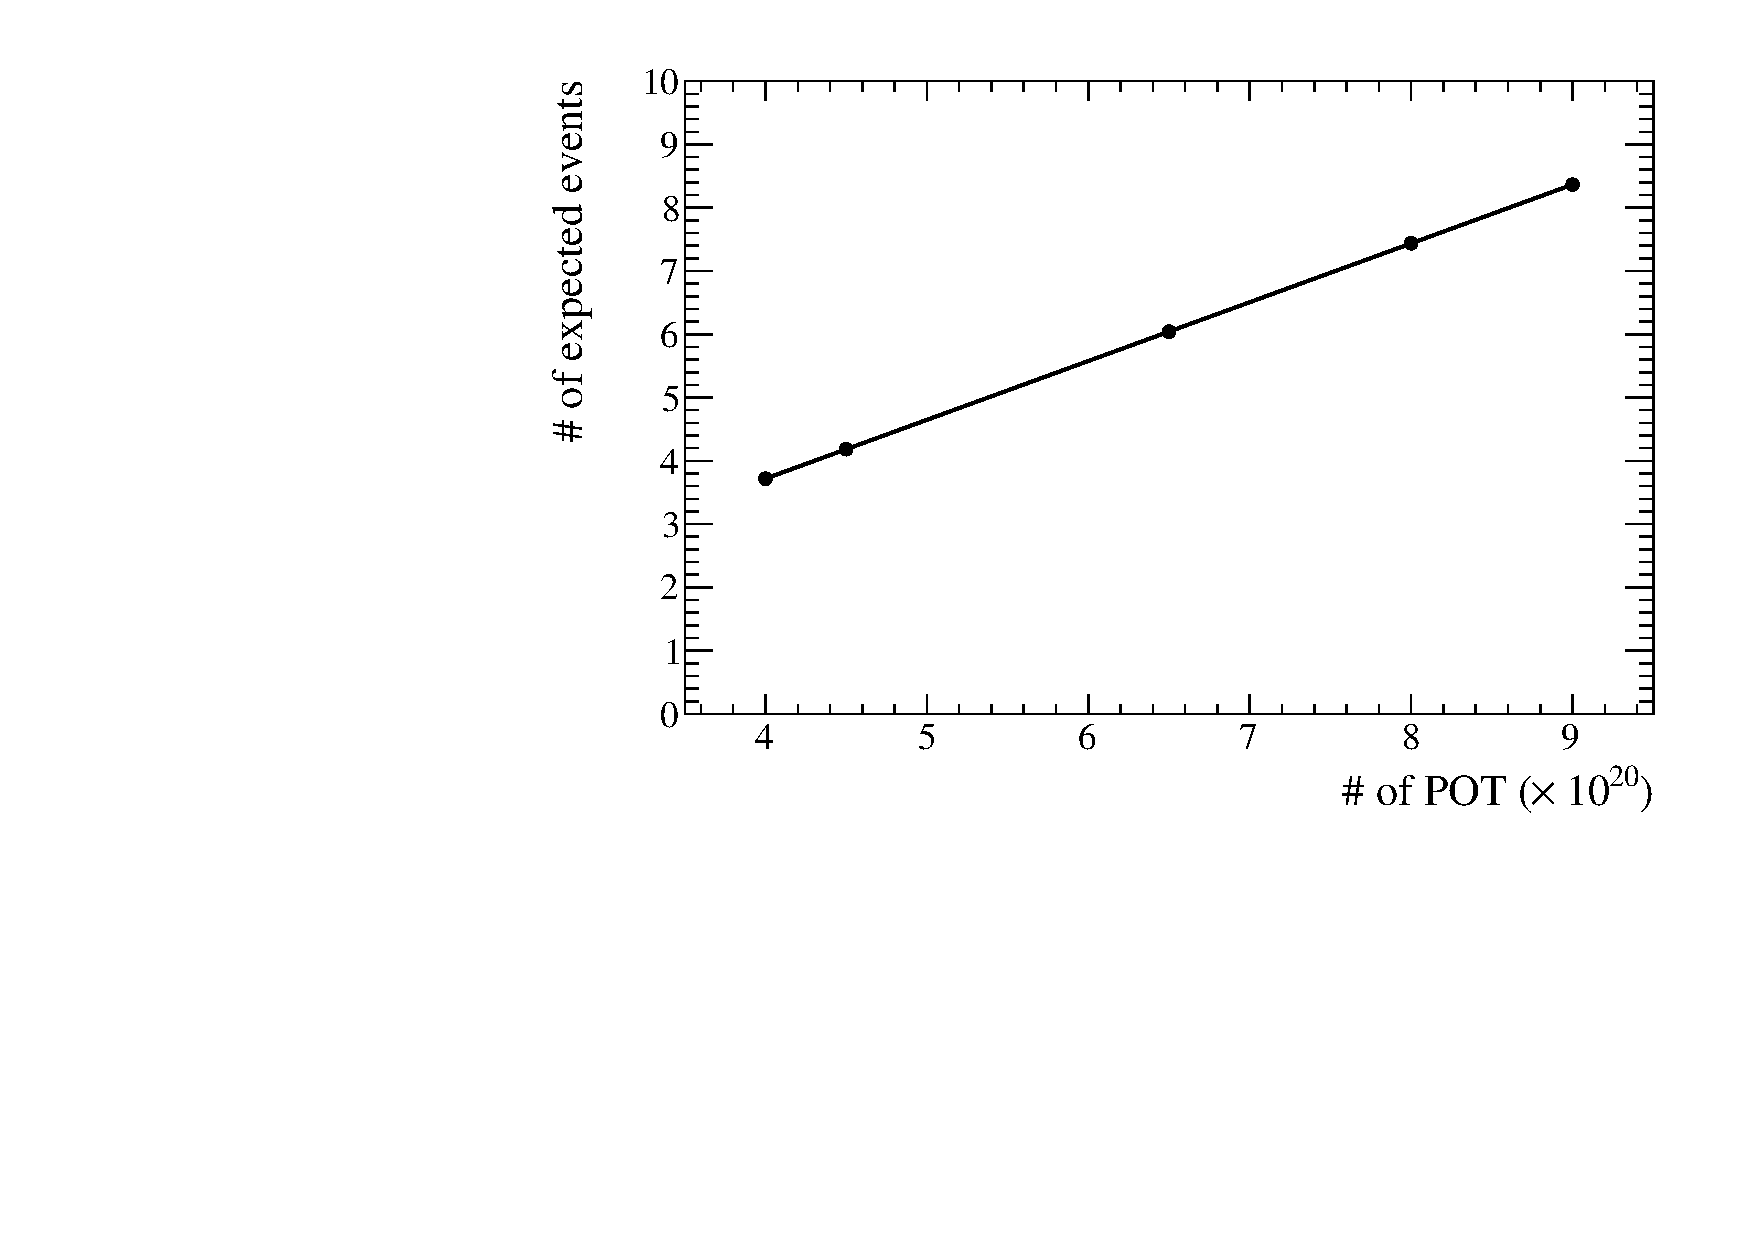
\includegraphics[width=0.48\linewidth]{./nuebar_plots/sensitivity/future_sensi/nobs_Vs_pot.pdf}
\caption {
The number of expected events is shown for different POT:
\FakePotLow POT, \FakePotHigh POT,
$6.5 \times 10^{20}$ POT, $8.0 \times 10^{20}$ POT and $9.0 \times 10^{20}$ POT.
The used oscillation parameters are shown in table~\ref{tab:osc_params_fixed_values_reactor}.
\NumToys toys are used.
}
\label{fig:sensi_future_nobs}
\end{figure}

\begin{figure}
\center
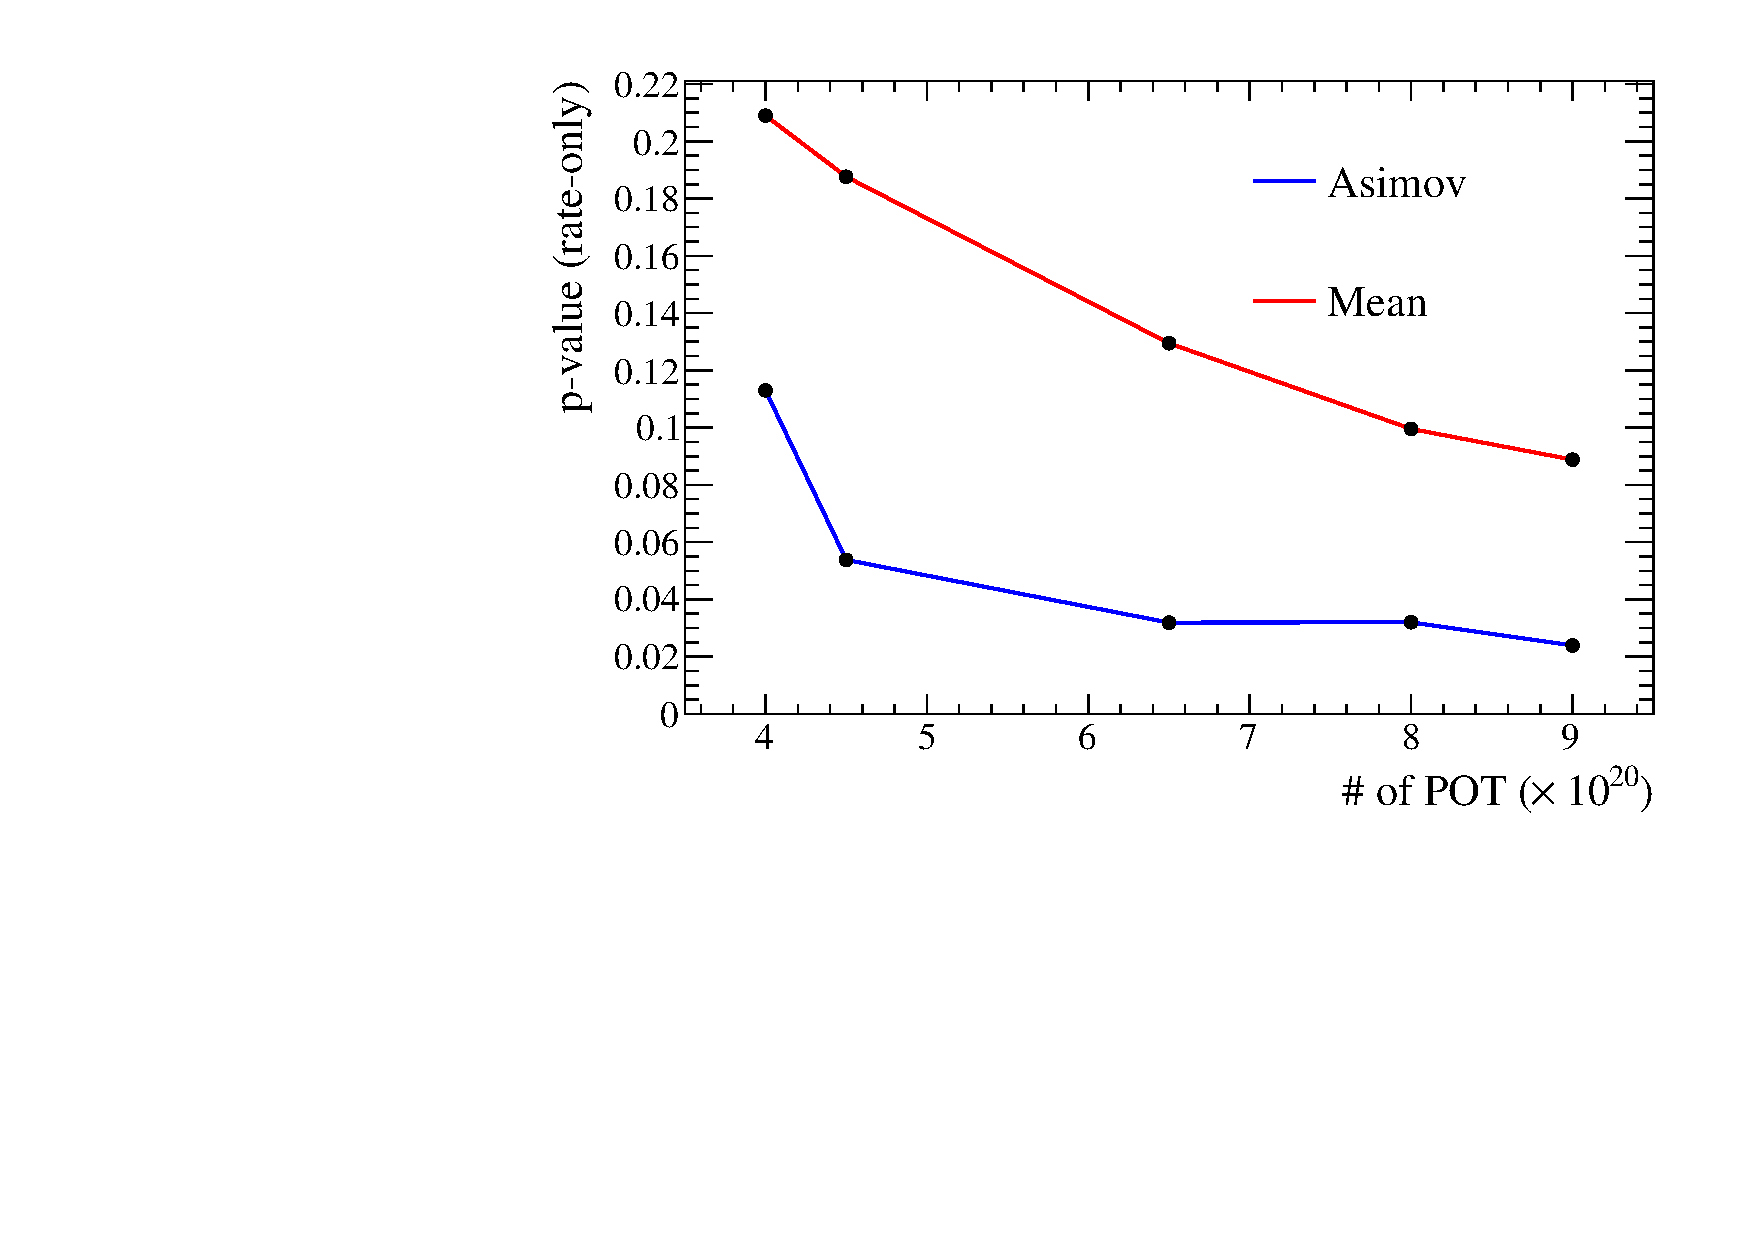
\includegraphics[width=0.48\linewidth]{./nuebar_plots/sensitivity/future_sensi/pvalue_Vs_pot_rate.pdf}
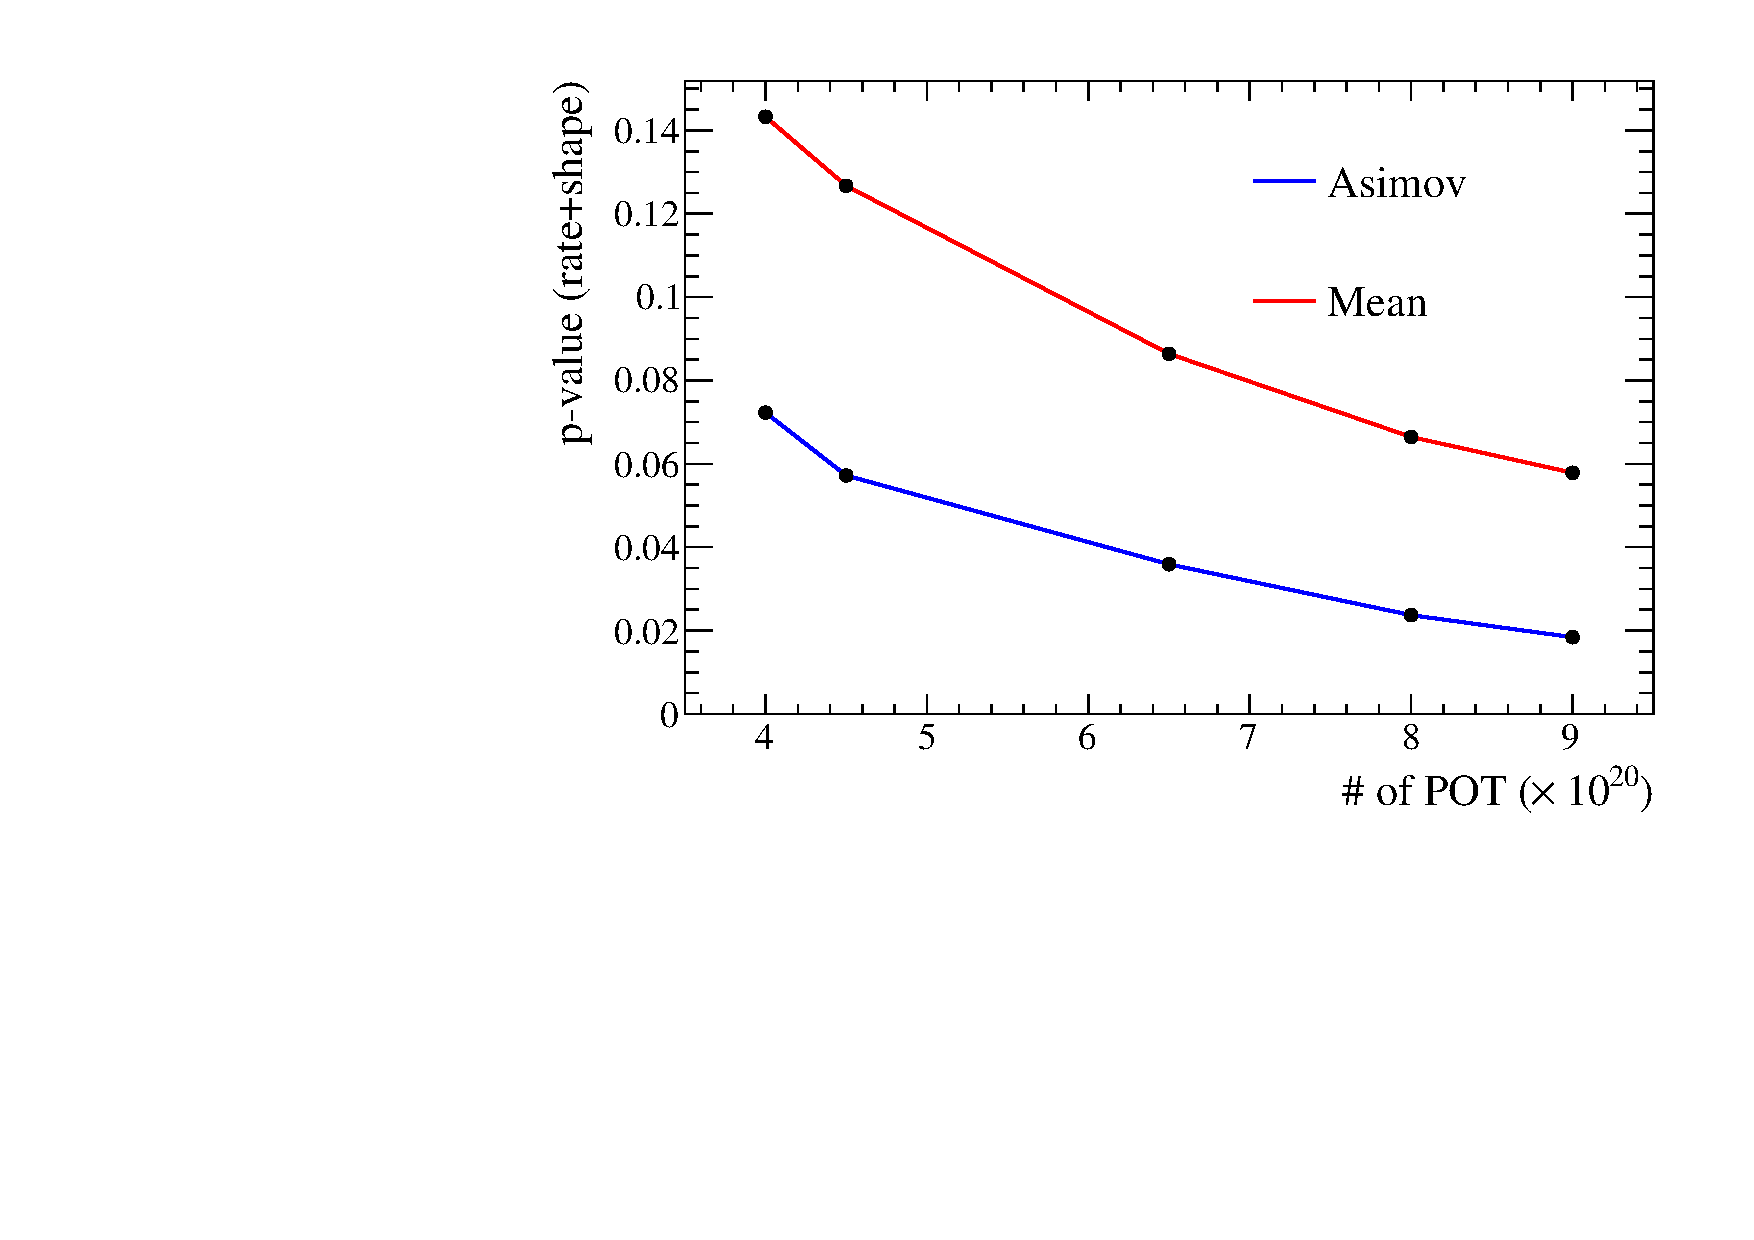
\includegraphics[width=0.48\linewidth]{./nuebar_plots/sensitivity/future_sensi/pvalue_Vs_pot_shape.pdf}
\caption {
The number of expected rate-only (left) and rate+shape (right) p-values are shown for different POT:
\FakePotLow POT, \FakePotHigh POT,
$6.5 \times 10^{20}$ POT, $8.0 \times 10^{20}$ POT and $9.0 \times 10^{20}$ POT.
\NumToys toys are used.
}
\label{fig:sensi_future_pvalue}
\end{figure}








\clearpage


